\documentclass[14pt, a4 paper]{article}
\usepackage{graphicx} % Required for inserting images

\usepackage[utf8]{inputenc}
\usepackage[T1]{fontenc}
\DeclareMathSymbol{\invques}{\mathord}{operators}{`>}
\DeclareUnicodeCharacter{00BF}{\tmquestiondown}
\DeclareRobustCommand{\tmquestiondown}{%
  \ifmmode\invques\else\textquestiondown\fi
}
\usepackage[portuges]{babel}%Babel -- irá activar automaticamente as regras apropriadas de hifenização para a língua todo o
                                   %-- o texto gerado é automaticamente traduzido para Português.
                                   %  Por exemplo, “chapter” irá passar a “capítulo”, “table of contents” a “conteúdo”.
                                   % portuges -- específica para o Português.
\usepackage[utf8]{inputenc} % define o encoding usado texto fonte (input)--usual "utf8" ou "latin1
\usepackage{parcolumns}

\usepackage{graphicx} %permite incluir graficos, tabelas, figuras
\usepackage{url} % para utilizar o comando \url{}
\usepackage{enumerate} %permite escolher, nas listas enumeradas, se os iems sao marcados com letras ou numeros-romanos em vez de numeracao normal

%\usepackage{apalike} % gerar biliografia no estilo 'named' (apalike)

\usepackage{color} % Para escrever em cores
\usepackage{multirow} %tabelas com multilinhas
\usepackage{array} %formatação especial de tabelas em array
\usepackage[pdftex]{hyperref} % transformar as referências internas do seu documento em hiper-ligações.
\usepackage{listings}
\usepackage{xcolor}
\definecolor{codegreen}{rgb}{0,0.6,0}
\definecolor{codegray}{rgb}{0.5,0.5,0.5}
\definecolor{codepurple}{rgb}{0.58,0,0.82}
\definecolor{backcolour}{rgb}{0.95,0.95,0.92}

\lstdefinestyle{mystyle}{
    backgroundcolor=\color{backcolour},   
    commentstyle=\color{codegreen},
    keywordstyle=\color{magenta},
    numberstyle=\tiny\color{codegray},
    stringstyle=\color{codepurple},
    basicstyle=\ttfamily\footnotesize,
    breakatwhitespace=false,         
    breaklines=true,                 
    captionpos=b,                    
    keepspaces=true,                 
    numbers=left,                    
    numbersep=5pt,                  
    showspaces=false,                
    showstringspaces=false,
    showtabs=false,                  
    tabsize=2
}

\lstset{style=mystyle}

%Exemplos de fontes -- nao e vulgar mudar o tipo de fonte
%\usepackage{tgbonum} % Fonte de letra: TEX Gyre Bonum
%\usepackage{lmodern} % Fonte de letra: Latin Modern Sans Serif
%\usepackage{helvet}  % Fonte de letra: Helvetica
%\usepackage{charter} % Fonte de letra:Charter

\definecolor{saddlebrown}{rgb}{0.55, 0.27, 0.07} % para definir uma nova cor, neste caso 'saddlebrown'

\usepackage{listings}  % para utilizar blocos de texto verbatim no estilo 'listings'
%paramerização mais vulgar dos blocos LISTING - GENERAL
\lstset{
	basicstyle=\small, %o tamanho das fontes que são usadas para o código
	numbers=left, % onde colocar a numeração da linha
	numberstyle=\tiny, %o tamanho das fontes que são usadas para a numeração da linha
	numbersep=5pt, %distancia entre a numeração da linha e o codigo
	breaklines=true, %define quebra automática de linha
    frame=tB,  % caixa a volta do codigo
	mathescape=true, %habilita o modo matemático
	escapeinside={(*@}{@*)} % se escrever isto  aceita tudo o que esta dentro das marcas e nao altera
}
%
%\lstset{ %
%	language=Java,							% choose the language of the code
%	basicstyle=\ttfamily\footnotesize,		% the size of the fonts that are used for the code
%	keywordstyle=\bfseries,					% set the keyword style
%	%numbers=left,							% where to put the line-numbers
%	numberstyle=\scriptsize,				% the size of the fonts that are used for the line-numbers
%	stepnumber=2,							% the step between two line-numbers. If it's 1 each line
%											% will be numbered
%	numbersep=5pt,							% how far the line-numbers are from the code
%	backgroundcolor=\color{white},			% choose the background color. You must add \usepackage{color}
%	showspaces=false,						% show spaces adding particular underscores
%	showstringspaces=false,					% underline spaces within strings
%	showtabs=false,							% show tabs within strings adding particular underscores
%	frame=none,								% adds a frame around the code
%	%abovecaptionskip=-.8em,
%	%belowcaptionskip=.7em,
%	tabsize=2,								% sets default tabsize to 2 spaces
%	captionpos=b,							% sets the caption-position to bottom
%	breaklines=true,						% sets automatic line breaking
%	breakatwhitespace=false,				% sets if automatic breaks should only happen at whitespace
%	title=\lstname,							% show the filename of files included with \lstinputlisting;
%											% also try caption instead of title
%	escapeinside={\%*}{*)},					% if you want to add a comment within your code
%	morekeywords={*,...}					% if you want to add more keywords to the set
%}

\usepackage{xspace} % deteta se a seguir a palavra tem uma palavra ou um sinal de pontuaçao se tiver uma palavra da espaço, se for um sinal de pontuaçao nao da espaço

\parindent=2pt %espaço a deixar para fazer a  indentação da primeira linha após um parágrafo
\parskip=4pt % espaço entre o parágrafo e o texto anterior

\setlength{\oddsidemargin}{-1cm} %espaço entre o texto e a margem
\setlength{\textwidth}{18cm} %Comprimento do texto na pagina
\setlength{\headsep}{-1cm} %espaço entre o texto e o cabeçalho
\setlength{\textheight}{23cm} %altura do texto na pagina

% comando '\def' usado para definir abreviatura (macros)
% o primeiro argumento é o nome do novo comando e o segundo entre chavetas é o texto original, ou sequência de controle, para que expande
\def\darius{\textsf{Darius}\xspace}
\def\antlr{\texttt{AnTLR}\xspace}
\def\titulo#1{\section{#1}}    %no corpo do documento usa-se na forma '\titulo{MEU TITULO}'
\def\super#1{{\em Supervisor: #1}\\ }
\def\area#1{{\em \'{A}rea: #1}\\[0.2cm]}
\def\resumo{\underline{Resumo}:\\ }
\def\e#1{\emph{#1}}


\title{Computação Gráfica (3º ano de LCC)\\
       \textbf{Trabalho Prático (Fase 1) — Grupo 1}\\ Relatório de Desenvolvimento}
\author{ Bruno Dias da Gião  (A96544) 
    \and Bruno Miguel Fernandes Araújo (A97509)
    \and João Luís da Cruz Pereira (A95375)}
\date{\today} %data

\begin{document}

\begin{titlepage}
\maketitle
\end{titlepage}

\tableofcontents
\listoffigures
\newpage
\section{Introdução} \label{chap:intro}

Este relatório serve como um apoio ao trabalho ,tem explicações sobre os raciocínios usados na primeira fase do projeto da unidade curricular Computação Gráfica.

Nesta fase tivemos de definir duas aplicações:

\begin{itemize}
\item{\textit{generator}}: que após a receção dos parâmetros necessários para a criação de um modelo, cria um ficheiro com a representação dos vértices deste modelo; 

\item {\textit{engine}}: que, a partir de um ficheiro de configuração, escrito em \textit{XML}, desenha um espaço com os modelos que já foram previamente gerados.
\end{itemize}
Demos uso dos módulos \textit{tinyxml2} para a leitura do ficheiro de configuração e do \textit{GLUT} para a representação gráfica.


\subsection{Estrutura do Relatório}
\begin{itemize}
\item \S\ref{chap:generator}- Descrevemos a implementação da aplicação \textit{generator}.

\item \S\ref{chap:engine} - Apresentamos a implementação da aplicação \textit{engine}. 

\item \S\ref{chap:conclusion} - Conclusão.

\item \S\ref{chap:resultado} - Imagens tiradas dos modelos gerados a partir dos ficheiros \textit{XML} dos testes e um exemplo.
\end{itemize}
\section{\textit{Generator}} \label{chap:generator}
Esta aplicação foi desenvolvida com o objetivo de gerar ficheiros do formato \textit{.3d} que serão eventualmente usados pela aplicação \textit{engine}.

O generator é capaz de gerar modelos para cinto tipos de primitivas, uma delas como extra, a torus.

Começaremos por analisar individualmente o raciocíno por detrás destas:
\subsection{Sphere}
Para a definição de uma esfera são necessários os seguintes parâmetros:

\begin{itemize}
\item O seu raio (\textit{radius});

\item O número de divisões verticais (\textit{slices});

\item O número de divisões horizontais (\textit{stacks});

\item O ficheiro que será aberto (\textit{file}).
\end{itemize}

Como variáveis iniciais temos:
\begin{itemize}
\item As coordenadas do ponto que foram calculadas (\textit{px},\textit{py},\textit{pz}).

\item $\alpha$, $\beta$ (inicializadas a 0) e as diferenças de $\alpha$ e $\beta$ que serão necessárias nos 
cálculos dos pontos.\\
Respetivamente, \textit{alpha}, \textit{beta} ,\textit{alpha\_diff}, \textit{beta\_diff}.

\item{alpha\_diff} é inicializado com a divisão entre o intervalo deste ($360^{\circ}$) e o número de slices.

\item{beta\_diff} é inicializado com a divisão entre o intervalo deste ($180^{\circ}$) e o número de stacks.

\end{itemize}
\begin{lstlisting} 
int32_t gen_sphere(float radius, int32_t slices, int32_t stacks, char*file)
{
	FILE* output = fopen(file, "w+");
	char buff[512];
	float px, py, pz, alpha_diff = 2 * M_PI / slices,
	      beta_diff = M_PI / stacks, alpha = 0, beta = 0;
	size_t b_read;
\end{lstlisting}

Para o cálculo dos pontos temos dois ciclos, um que itera até o número de slices, que acaba na reatribuição de $0$ a beta e incrementando o valor de alpha com alpha\_ diff permitindo que alpha, ao longo deste ciclo, tenha todos os valores possíveis no seu intervalo de $360^{\circ}$.

Temos então um outro ciclo interno que itera até o número de stacks e terá os cálculos para 6 pontos (2 triângulos) que seguem a seguinte primitiva:
$$
px= radius \times \cos(\beta) \times \sin(\alpha)
$$
$$
py= radius \times \sin(\beta)
$$
$$
pz= radius \times \cos(\beta) \times \sin(\beta)
$$
Para termos então os pontos necessários iremos somar beta\_diff , alpha\_diff ou ambos dependendo do requerido e por fim incrementar a $\beta$, beta\_diff. É de notar que $\beta$ tem um decremento de 90º pois queremos que ao longo do ciclo este varie entre $-90<\beta<90$ tal como foi lecionado.

\verb|if(j!=0){}| e \verb|if(j!=stacks-1){}| foram necessários para evitar a sobreposição de triângulos, quando estamos no topo ou no fundo da esfera.

\begin{lstlisting}[language = c++]
	for (int i = 0; i < slices; i++) {
		for (int j = 0; j < stacks; j++) { /* ifs */
			if(j!=0){
				b_read = snprintf(buff, 512, "%.3f %.3f %.3f\n",
						  radius * cosf(beta - M_PI_2) * cosf(alpha),
						  radius * sinf(beta - M_PI_2),
						  radius*cosf(beta-M_PI_2)*sinf(alpha));
				fwrite(buff, sizeof (int8_t),b_read, output);
				b_read = snprintf(buff, 512, "%.3f %.3f %.3f\n",
						  radius * cosf(beta - M_PI_2 + beta_diff)
							* cosf(alpha + alpha_diff),
						  radius * sinf(beta - M_PI_2 + beta_diff),
						  radius*cosf(beta-M_PI_2+beta_diff)*
							sinf(alpha + alpha_diff));
				fwrite(buff, sizeof (int8_t),b_read, output);
				b_read = snprintf(buff, 512, "%.3f %.3f %.3f\n",
						  radius * cosf(beta - M_PI_2)
							* cosf(alpha + alpha_diff),
						  radius * sinf(beta - M_PI_2),
						  radius*cosf(beta-M_PI_2)
							*sinf(alpha + alpha_diff));
				fwrite(buff, sizeof (int8_t),b_read, output);
			}
			if(j!=stacks-1){
				b_read = snprintf(buff, 512, "%.3f %.3f %.3f\n",
						  radius * cosf(beta - M_PI_2) * cosf(alpha),
						  radius * sinf(beta - M_PI_2),
						  radius*cosf(beta-M_PI_2)*sinf(alpha));
				fwrite(buff, sizeof (int8_t),b_read, output);
				b_read = snprintf(buff, 512, "%.3f %.3f %.3f\n",
						  radius * cosf(beta - M_PI_2 + beta_diff) * cosf(alpha),
						  radius * sinf(beta - M_PI_2 + beta_diff),
						  radius*cosf(beta-M_PI_2 + beta_diff)*sinf(alpha));
				fwrite(buff, sizeof (int8_t),b_read, output);
				b_read = snprintf(buff, 512, "%.3f %.3f %.3f\n",
						  radius * cosf(beta - M_PI_2 + beta_diff)
							* cosf(alpha + alpha_diff),
						  radius * sinf(beta - M_PI_2 + beta_diff),
						  radius*cosf(beta-M_PI_2+beta_diff)*
							sinf(alpha + alpha_diff));
				fwrite(buff, sizeof (int8_t),b_read, output);
			}
			beta += beta_diff;
		}
		beta = 0;
		alpha += alpha_diff;
	}
	fclose(output);
	return 0;
}
\end{lstlisting}

\subsection{Cone}
Para a definição de um cone são necessários os seguintes parâmetros:

\begin{itemize}
\item O raio da sua base (\textit{radius}).

\item A sua altura (\textit{height}).

\item O número de divisões verticais (\textit{slices}).

\item O número de divisões horizontais (\textit{stacks}).

\item Por fim o ficheiro que será aberto (\textit{file}).
\end{itemize}

Para o cálculo dos pontos da figura começamos por ter dois \textit{nested loops} onde percorremos cada \textit{stack} (nível) e todas as \textit{slices} no mesmo. Começamos por desenhar a base que será composta por um triângulo por cada slice. Os pontos são calculados através de coordenadas polares com centro na origem e a diferença de ângulo entre cada slice é obtido através da divisão do ângulo total pelo número de slices.
Ou seja, 
$$ 
px = rad \times \sin(\alpha)
$$
$$
pz = rad \times \cos(\alpha)
$$

Analisando agora o caso de ser a última \textit{stack} será apenas um triângulo que liga ao centro com a altura desejada, o método de calcular as coordenadas é o mesmo que na base.  

No caso de não ser a última \textit{stack} (base e restantes stacks) iremos querer desenhar um quadrado composto por $2$ triângulos. Os mesmos são obtidos da mesma forma que as restantes coordenadas mas tendo em conta a diferença no valor do \textit{y} para além da diferença do ângulo.

No final de cada iteração do ciclo mais interior, o ângulo é incrementado por \textit{angle\_diff}.
No caso do ciclo exterior, o ângulo volta a $0$, o valor de \textit{y} é incrementado por \textit{y\_diff} (valor da altura dividido pelo número de stacks) e o raio é decrementado por \textit{xz\_diff} (valor do raio dividido pelo número de stacks).

\begin{lstlisting}[language = c++]
int32_t gen_cone(float radius, float height, int32_t slices, int32_t stacks, char*file)
{
FILE* output = fopen(file, "w+");
char buff[512];
size_t b_read;
int i, j, r = 0;
float y=0;
float angle = 0;
float cur_rad = radius;
float angle_diff = 2*M_PI/slices;
float xz_diff = radius/stacks;
float y_diff = height/stacks;

for(i=0; i<stacks; i++) {
    for(j=0; j<slices; j++) {
        // Bottom face
        if (i==0) {
            b_read = snprintf(buff, 512, "%.3f %.3f %.3f\n", cur_rad*sinf(angle), 0.f, cur_rad*cosf(angle));
            fwrite(buff, sizeof (int8_t),b_read, output);
            b_read = snprintf(buff, 512, "%.3f %.3f %.3f\n", 0.f, 0.f, 0.f);
            fwrite(buff, sizeof (int8_t),b_read, output);
            b_read = snprintf(buff, 512, "%.3f %.3f %.3f\n", cur_rad*sinf(angle+angle_diff), 0.f, cur_rad*cosf(angle+angle_diff));
            fwrite(buff, sizeof (int8_t),b_read, output);
        }
       
        if (i==stacks-1){              
            b_read = snprintf(buff, 512, "%.3f %.3f %.3f\n", cur_rad*sinf(angle+angle_diff), y, cur_rad*cosf(angle+angle_diff));
            fwrite(buff, sizeof (int8_t),b_read, output);
            b_read = snprintf(buff, 512, "%.3f %.3f %.3f\n", 0.f, height, 0.f);
            fwrite(buff, sizeof (int8_t),b_read, output);
            b_read = snprintf(buff, 512, "%.3f %.3f %.3f\n", cur_rad*sinf(angle), y, cur_rad*cosf(angle));
            fwrite(buff, sizeof (int8_t),b_read, output);
        }
        else {
            b_read = snprintf(buff, 512, "%.3f %.3f %.3f\n", (cur_rad-xz_diff)*sinf(angle+angle_diff), y+y_diff,
                      (cur_rad-xz_diff)*cosf(angle+angle_diff));
            fwrite(buff, sizeof (int8_t),b_read, output);
            b_read = snprintf(buff, 512, "%.3f %.3f %.3f\n", (cur_rad-xz_diff)*sinf(angle), y+y_diff,
                      (cur_rad-xz_diff)*cosf(angle));
            fwrite(buff, sizeof (int8_t),b_read, output);
            b_read = snprintf(buff, 512, "%.3f %.3f %.3f\n", cur_rad*sinf(angle+angle_diff), y,
                      cur_rad*cosf(angle+angle_diff));
            fwrite(buff, sizeof (int8_t),b_read, output);

            b_read = snprintf(buff, 512, "%.3f %.3f %.3f\n", (cur_rad-xz_diff)*sinf(angle), y+y_diff,
                      (cur_rad-xz_diff)*cosf(angle));
            fwrite(buff, sizeof (int8_t),b_read, output);
            b_read = snprintf(buff, 512, "%.3f %.3f %.3f\n", cur_rad*sinf(angle), y,
                      cur_rad*cosf(angle));
            fwrite(buff, sizeof (int8_t),b_read, output);
            b_read = snprintf(buff, 512, "%.3f %.3f %.3f\n", cur_rad*sinf(angle+angle_diff), y,
                      cur_rad*cosf(angle+angle_diff));
            fwrite(buff, sizeof (int8_t),b_read, output);
        }
        angle += angle_diff;
    }
    angle = 0;
    y += y_diff;
    cur_rad -= xz_diff;
}
fclose(output);
return r;
}
\end{lstlisting}

\subsection{Plane}
Para a definição de um \textit{Plane} são necessários os seguintes parâmetros:
\begin{itemize}
\item O seu comprimento (\textit{full\_size}).

\item O número de divisões (\textit{divs}).

\item Por fim o ficheiro que será aberto (\textit{file}).
\end{itemize}

Começamos por ter dois \textit{nested loops} cada um a percorrer o número de divisões que o plano tem (pois o mesmo será quadrado). Por cada iteração teremos um quadrado composto por dois triângulos.

Começamos com o \textit{x} a metade do comprimento e o \textit{z} como o inverso de \textit{x}, ou seja, o inverso da metade do comprimento. Teremos então, como ponto inicial, o ponto com o maior valor de x e o menor valor de z.

Em cada iteração do ciclo mais interior iremos calcular os pontos através da somas e subtração de \textit{off} (comprimento a dividir pelo número de divisões). No final, subtraímos o valor de \textit{off} ao \textit{x} para passarmos para o próximo quadrado a ser desenhado.

No final de cada iteração do ciclo mais exterior, voltamos a colocar o valor de \textit{x} como metade do comprimento (voltar ao início) e incrementamos o \textit{z} por \textit{off} (próxima linha de quadrados).

\begin{lstlisting}[language=c++]
int32_t gen_plane(float full_size, int32_t divs, char* file)
{
	FILE* output = fopen(file, "w+"); 
	char buff[512];
	size_t b_read;
	float x = full_size/2, z = -x, off=full_size/divs;
	int i,j, err = 0;

	for (i=0; i < divs; i++) {
		for (j=0; j < divs; j++) {
			//curr.x = x = i * div_len - div_len + off;
			b_read = sprintf(buff, "%.3f 0.000 %.3f\n", x, z+off);
			fwrite(buff, sizeof (int8_t),b_read, output);

			b_read = sprintf(buff, "%.3f 0.000 %.3f\n", x, z);
			fwrite(buff, sizeof (int8_t),b_read, output);
			
			b_read = sprintf(buff, "%.3f 0.000 %.3f\n", x-off, z);
			fwrite(buff, sizeof (int8_t),b_read, output);

			b_read = sprintf(buff, "%.3f 0.000 %.3f\n", x-off, z);
			fwrite(buff, sizeof (int8_t),b_read, output);
			
			b_read = sprintf(buff, "%.3f 0.000 %.3f\n", x-off, z+off);
			fwrite(buff, sizeof (int8_t),b_read, output);

			b_read = sprintf(buff, "%.3f 0.000 %.3f\n", x, z+off);
			fwrite(buff, sizeof (int8_t),b_read, output);

			x -= off;
		}
		x = full_size/ 2;
		z += off;
	}

	fclose(output);
	return err;
}
\end{lstlisting}

\begin{lstlisting}[language=c++]

\end{lstlisting}

\subsection{Box}
Para a definição de uma box são necessários os seguintes parâmetros:

\begin{itemize}
    \item O seu comprimento (\textit{l}).
    \item O número de divisões para cada aresta (\textit{d})
    \item Por fim o ficheiro que será aberto (\textit{file}).

\end{itemize}

Seguindo um raciocínio similar ao plano, iremos fazer novamente dois \textit{nested loops} sobre as mesmas circunstâncias mas desta vez para cada duas faces da \textit{Box}.

Começamos pela base e o pelo topo da \textit{Box}, faces paralelas ao plano \textit{x0z}.

Seguidamente a face de trás e da frente, faces paralelas ao plano \textit{y0x}.

Por fim a face da direita e da esquerda, faces paralelas ao plano \textit{y0z}.

Apesar de realmente ter cálculos diferentes, o raciocínio por detrás deste é similar ao do plane.

\begin{lstlisting}[language=c++]
int32_t gen_box(float l, int32_t d, char* file) 
{
	FILE* output = fopen(file, "w+");
	char buff[512];
	size_t b_read;
	int32_t i, j, r = 0;
	float x = -l/2;
	float y = l/2;
	float z = -l/2;
	float diff = l/d;

    // Bottom and Top Faces
	for (i=0; i<d; i++){
		for (j=0; j<d; j++) {
			

			b_read = snprintf(buff, 512, "%.3f %.3f %.3f\n", x, y, z);
			fwrite(buff, sizeof (int8_t),b_read, output);
			b_read = snprintf(buff, 512, "%.3f %.3f %.3f\n", x+diff, y, z+diff);
			fwrite(buff, sizeof (int8_t),b_read, output);
			b_read = snprintf(buff, 512, "%.3f %.3f %.3f\n", x+diff, y, z);
			fwrite(buff, sizeof (int8_t),b_read, output);

			b_read = snprintf(buff, 512, "%.3f %.3f %.3f\n", x, y, z);
			fwrite(buff, sizeof (int8_t),b_read, output);
			b_read = snprintf(buff, 512, "%.3f %.3f %.3f\n", x, y, z+diff);
			fwrite(buff, sizeof (int8_t),b_read, output);
			b_read = snprintf(buff, 512, "%.3f %.3f %.3f\n", x+diff, y, z+diff);
			fwrite(buff, sizeof (int8_t),b_read, output);

			b_read = snprintf(buff, 512, "%.3f %.3f %.3f\n", x+diff, -y, z+diff);
			fwrite(buff, sizeof (int8_t),b_read, output);
			b_read = snprintf(buff, 512, "%.3f %.3f %.3f\n", x, -y, z);
			fwrite(buff, sizeof (int8_t),b_read, output);
			b_read = snprintf(buff, 512, "%.3f %.3f %.3f\n", x+diff,-y, z);
			fwrite(buff, sizeof (int8_t),b_read, output);

			b_read = snprintf(buff, 512, "%.3f %.3f %.3f\n", x, -y, z+diff);
			fwrite(buff, sizeof (int8_t),b_read, output);
			b_read = snprintf(buff, 512, "%.3f %.3f %.3f\n", x, -y, z);
			fwrite(buff, sizeof (int8_t),b_read, output);
			b_read = snprintf(buff, 512, "%.3f %.3f %.3f\n", x+diff, -y, z+diff);
			fwrite(buff, sizeof (int8_t),b_read, output);

			z += diff;
		}
		z = - l/2;
		x += diff;
	}

	x = -l / 2;
	y = -l / 2;
	z = l / 2;

    // Front and Back faces
	for (int i=0; i<d; i++){
		for (int j=0; j<d; j++) {

			b_read = snprintf(buff, 512, "%.3f %.3f %.3f\n", x+diff, y+diff, z);
			fwrite(buff, sizeof (int8_t),b_read, output);
			b_read = snprintf(buff, 512, "%.3f %.3f %.3f\n", x, y, z);
			fwrite(buff, sizeof (int8_t),b_read, output);
			b_read = snprintf(buff, 512, "%.3f %.3f %.3f\n", x+diff, y, z);
			fwrite(buff, sizeof (int8_t),b_read, output);

			b_read = snprintf(buff, 512, "%.3f %.3f %.3f\n", x, y+diff, z);
			fwrite(buff, sizeof (int8_t),b_read, output);
			b_read = snprintf(buff, 512, "%.3f %.3f %.3f\n", x, y, z);
			fwrite(buff, sizeof (int8_t),b_read, output);
			b_read = snprintf(buff, 512, "%.3f %.3f %.3f\n", x+diff, y+diff, z);
			fwrite(buff, sizeof (int8_t),b_read, output);

			b_read = snprintf(buff, 512, "%.3f %.3f %.3f\n", x, y, -z);
			fwrite(buff, sizeof (int8_t),b_read, output);
			b_read = snprintf(buff, 512, "%.3f %.3f %.3f\n", x+diff, y+diff, -z);
			fwrite(buff, sizeof (int8_t),b_read, output);
			b_read = snprintf(buff, 512, "%.3f %.3f %.3f\n", x+diff, y, -z);
			fwrite(buff, sizeof (int8_t),b_read, output);

			b_read = snprintf(buff, 512, "%.3f %.3f %.3f\n", x, y, -z);
			fwrite(buff, sizeof (int8_t),b_read, output);
			b_read = snprintf(buff, 512, "%.3f %.3f %.3f\n", x, y+diff, -z);
			fwrite(buff, sizeof (int8_t),b_read, output);
			b_read = snprintf(buff, 512, "%.3f %.3f %.3f\n", x+diff, y+diff, -z);
			fwrite(buff, sizeof (int8_t),b_read, output);

			y += diff;
		}
		y = -l/2;
		x += diff;
	}
    
	z = - l/2;
	y = - l/2;
	x = l/2;

    // Right and Left faces
	for (int i=0; i<d; i++){
		for (int j=0; j<d; j++) {

			b_read = snprintf(buff, 512, "%.3f %.3f %.3f\n", x, y, z);
			fwrite(buff, sizeof (int8_t),b_read, output);
			b_read = snprintf(buff, 512, "%.3f %.3f %.3f\n", x, y+diff, z+diff);
			fwrite(buff, sizeof (int8_t),b_read, output);
			b_read = snprintf(buff, 512, "%.3f %.3f %.3f\n", x, y, z+diff);
			fwrite(buff, sizeof (int8_t),b_read, output);

			b_read = snprintf(buff, 512, "%.3f %.3f %.3f\n", x, y, z);
			fwrite(buff, sizeof (int8_t),b_read, output);
			b_read = snprintf(buff, 512, "%.3f %.3f %.3f\n", x, y+diff, z);
			fwrite(buff, sizeof (int8_t),b_read, output);
			b_read = snprintf(buff, 512, "%.3f %.3f %.3f\n", x, y+diff, z+diff);
			fwrite(buff, sizeof (int8_t),b_read, output);

			b_read = snprintf(buff, 512, "%.3f %.3f %.3f\n", -x, y+diff, z+diff);
			fwrite(buff, sizeof (int8_t),b_read, output);
			b_read = snprintf(buff, 512, "%.3f %.3f %.3f\n", -x, y, z);
			fwrite(buff, sizeof (int8_t),b_read, output);
			b_read = snprintf(buff, 512, "%.3f %.3f %.3f\n", -x, y, z+diff);
			fwrite(buff, sizeof (int8_t),b_read, output);

			b_read = snprintf(buff, 512, "%.3f %.3f %.3f\n", -x, y+diff, z);
			fwrite(buff, sizeof (int8_t),b_read, output);
			b_read = snprintf(buff, 512, "%.3f %.3f %.3f\n", -x, y, z);
			fwrite(buff, sizeof (int8_t),b_read, output);
			b_read = snprintf(buff, 512, "%.3f %.3f %.3f\n", -x, y+diff, z+diff);
			fwrite(buff, sizeof (int8_t),b_read, output);

			y += diff;
		}
		y = -l/2;
		z += diff;
	}

	fclose(output);
	return 0;
}
\end{lstlisting}

\subsection{Torus}
Para a definição de um torus são necessários os seguintes parâmetros:

\begin{itemize}
\item O raio interno (\textit{inner\_radius}).

\item O raio externo (\textit{outer\_radius}).

\item O número de divisões verticais(\textit{slices}).

\item O número de divisões horizontais(\textit{stacks}).

\item Por fim o ficheiro que será aberto (\textit{file}).
\end{itemize}
Para o cálculo dos pontos utilizamos dois \textit{nested loops}, um para cada slice, e outro para cada stack.
Para obtermos as coordenadas dos pontos utilizamos:
$$
px = (inner_radius + outer_radius * cos(beta - \pi) * cos(alfa)
$$
$$
py = outer_radius*sin(beta - \pi)
$$
$$
pz = (inner_radius + outer_radius * cos(beta - \pi)) * sin(alfa)
$$

Utilizamos também a diferença entre cada \textit{slice} para calcular a diferença entre cada \textit{beta} e a diferença entre \textit{stacks} para calcular a diferença entre cada \textit{alfa}.

No final de cada iteração do ciclo mais interior incrementamos o beta por \textit{beta\_diff}. No caso do ciclo mais exterior o \textit{beta} é colocado a $0$ e o alfa é incrementado por \textit{alfa\_diff}.

\begin{lstlisting}[language = c++]
int32_t gen_torus(float inner_radius, float outer_radius,
		  int32_t slices, int32_t stacks, char* file)
{
	FILE* output = fopen(file, "w+");
	float alfa = 0, beta = 0;
	float alfa_diff = 2 * M_PI / slices;
	float beta_diff = 2*M_PI / stacks;
	float px, py, pz;
	char buff[512];
	size_t b_read;
	int32_t rr = 0;

	for (int i = 0; i < slices; i++) {
		for (int j = 0; j < stacks; j++) {

			px = (inner_radius + outer_radius * cos(beta -M_PI_2)) * cos(alfa);
			py = outer_radius * sin(beta - M_PI_2);
			pz = (inner_radius + outer_radius * cos(beta - M_PI_2)) * sin(alfa);
			b_read = sprintf(buff, "%.3f %.3f %.3f\n", px, py, pz);
			fwrite(buff, sizeof (int8_t),b_read, output);

			px = (inner_radius + outer_radius * cos(beta - M_PI_2 + beta_diff)) * cos(alfa);
			py = outer_radius * sin(beta - M_PI_2+ beta_diff);
			pz = (inner_radius + outer_radius * cos(beta - M_PI_2 + beta_diff)) * sin(alfa);
			b_read = sprintf(buff, "%.3f %.3f %.3f\n", px, py, pz);
			fwrite(buff, sizeof (int8_t),b_read, output);

			px = (inner_radius + outer_radius * cos(beta - M_PI_2 )) * cos(alfa+alfa_diff);
			py =  outer_radius * sin(beta - M_PI_2);
			pz= (inner_radius + outer_radius * cos(beta - M_PI_2)) * sin(alfa+alfa_diff);
			b_read = sprintf(buff, "%.3f %.3f %.3f\n", px, py, pz);
			fwrite(buff, sizeof (int8_t),b_read, output);

			px = (inner_radius + outer_radius * cos(beta - M_PI_2 + beta_diff)) * cos(alfa);
			py =  outer_radius * sin(beta - M_PI_2 + beta_diff);
			pz = (inner_radius + outer_radius * cos(beta - M_PI_2 + beta_diff)) * sin(alfa);
			b_read = sprintf(buff, "%.3f %.3f %.3f\n", px, py, pz);
			fwrite(buff, sizeof (int8_t),b_read, output);

			px = (inner_radius + outer_radius * cos(beta - M_PI_2 + beta_diff)) * cos(alfa + alfa_diff);
			py =  outer_radius * sin(beta - M_PI_2 + alfa_diff);
			pz = (inner_radius +outer_radius * cos(beta - M_PI_2 + beta_diff)) * sin(alfa + alfa_diff);
			b_read = sprintf(buff, "%.3f %.3f %.3f\n", px, py, pz);
			fwrite(buff, sizeof (int8_t),b_read, output);

			px = (inner_radius + outer_radius * cos(beta - M_PI_2)) * cos(alfa + alfa_diff);
			py = outer_radius * sin(beta - M_PI_2);
			pz = (inner_radius + outer_radius * cos(beta - M_PI_2)) * sin(alfa + alfa_diff);
			b_read = sprintf(buff, "%.3f %.3f %.3f\n", px, py, pz);
			fwrite(buff, sizeof (int8_t),b_read, output);

			beta += beta_diff;
		}
		beta = 0;
		alfa += alfa_diff;
	
	}
	fclose(output);
	return rr;
}
\end{lstlisting}


\section{\textit{Engine}} \label{chap:engine}
Relativamente ao \textbf{Motor}, temos que 
\begin{enumerate}
    \item Fazemos \textit{parse} de um ficheiro XML que será o \textit{input} do nosso motor;
    \item Fazemos \textit{parse} das primitivas num \textit{path} fixo - \verb|/prims/|;
    \item Finalmente podemos inicializar o ambiente OpenGL e iniciar o ciclo principal do programa.
\end{enumerate}

Procederemos então a explicar cada uma destas fases detalhadamente.

\subsection{Parse do ficheiro XML}

Fazendo uso da biblioteca \textbf{tinyxml2} \footnote{ver \url{https://github.com/leethomason/tinyxml2}}, podemos extrair a informação dos atributos de cada elemento XML, que será onde, maioritariamente, se encontram as informações que desejamos. A informação de cada atributo \'e armazenada numa struct global
\verb|world| composta por structs representativas de cada elemento do \textit{input}.

De notar também o modo como são armazenados os nomes dos ficheiros .3d, isto é, num vetor de struct prims que é constituido por um nome, um contador de quantas vezes vai ser desenhado num dado grupo e que grupo constitui.  

Tamb\'em extendemos o XML com a possibilidade de, opcionalmente alterar o título da janela e a posição
inicial da janela (caso contr\'ario inicia com ``CG-PROJ'' - $0,0$, respetivamente).
\begin{lstlisting}[language = c++]
float alfa = 0.0f, beta = 0.0f, radius = 5.0f;
float camX, camY, camZ;
int timebase, time, frames=0;
float fps;
int cur_mode = GL_LINE, cur_face = GL_FRONT;
GLuint vertex_count, vertices;

struct triple {
	float x,y,z;
};
struct prims {
	int count;
	int group;
	char name[64];
};
struct {
	struct {
		int h,w,sx,sy;
		char title[64];
	} win;
	struct {
		struct triple pos;
		struct triple lookAt;
		struct triple up; /* 0 1 0 */
		struct triple proj; /* 60 1 1000*/
	} cam;
	std::vector<struct prims> primitives;
} world;

typedef std::vector<struct triple> Primitive_Coords;
std::vector<Primitive_Coords> prims;
static int not_in_prims_g(const char* f, int* i, int g, int N)
{
	int r = 1;
	for (*i=0; *i< N && r; *i+=1) {
		if (!strcmp(f, world.primitives[*i].name) &&
		    world.primitives[*i].group == g)
		    r = 0;
	}
	return r;
}

\end{lstlisting}
\begin{lstlisting}[language = c++]
int xml_init(char* xml_file)
{
	XMLDocument doc;
	XMLElement* world_l, *window, *cam, *posi, *lookAt, *up, *proj,
		*group_R, *gr, *mod, *models;
	int i = 0, g, j, rs = 0;
	const char* f;
	const char* tit;
	char tmp[1024];
	doc.LoadFile(xml_file);

	world_l = doc.RootElement();
	if (world_l) {
		window = world_l->FirstChildElement("window");
		if (!window) {
			return -1;
		}
		world.win.w = window->IntAttribute("width");
		world.win.h = window->IntAttribute("height");
		world.win.sx = 0;
		world.win.sy = 0;
		world.win.sx = window->IntAttribute("x");
		world.win.sy = window->IntAttribute("y");
		tit = window->Attribute("title");
		if (tit)
			strcpy(world.win.title, window->Attribute("title"));
		else
			strcpy(world.win.title, "CG-PROJ");
		cam = world_l->FirstChildElement("camera");
		if (!cam) {
			return -2;
		}
		posi = cam->FirstChildElement("position");
		if (!posi) {
			return -3;
		}
		world.cam.pos.x = posi->FloatAttribute("x");
		world.cam.pos.y = posi->FloatAttribute("y");
		world.cam.pos.z = posi->FloatAttribute("z");
		printf("%.3f %.3f %.3f\n", world.cam.pos.x,
		       world.cam.pos.y,
		       world.cam.pos.z);
		lookAt = cam->FirstChildElement("lookAt");
		if (!lookAt) {
			return -4;
		}
		world.cam.lookAt.x = lookAt->FloatAttribute("x");
		world.cam.lookAt.y = lookAt->FloatAttribute("y");
		world.cam.lookAt.z = lookAt->FloatAttribute("z");
		printf("%.3f %.3f %.3f\n", world.cam.lookAt.x,
		       world.cam.lookAt.y,
		       world.cam.lookAt.z);
		up = cam->FirstChildElement("up");
		if (up) {
			world.cam.up.x = up->FloatAttribute("x");
			world.cam.up.y = up->FloatAttribute("y");
			world.cam.up.z = up->FloatAttribute("z");
		}
		else {
			world.cam.up.x = 0.f;
			world.cam.up.y = 1.f;
			world.cam.up.z = 0.f;
		}
		printf("%.3f %.3f %.3f\n", world.cam.up.x,
		       world.cam.up.y,
		       world.cam.up.z);
		proj = cam->FirstChildElement("projection");
		if (proj) {
			world.cam.proj.x = proj->FloatAttribute("fov");
			world.cam.proj.y = proj->FloatAttribute("near");
			world.cam.proj.z = proj->FloatAttribute("far");
		}
		else {
			world.cam.proj.x = 60.f; // fov
			world.cam.proj.y = 1.f; // neAR
			world.cam.proj.z = 1000.f; //far
		}
		printf("%.3f %.3f %.3f\n", world.cam.proj.x,
		       world.cam.proj.y,
		       world.cam.proj.z);
		group_R = world_l->FirstChildElement("group");
		if (group_R){
			for (gr=group_R, g=0;
			     gr;
			     gr = gr->FirstChildElement("group"),
			     g += 1) {

				models = gr->FirstChildElement("models");
				if (models) {
					for (mod=models->FirstChildElement("model");
					     mod;
					     mod=mod->NextSiblingElement("model")
					     ) {

						if (mod){
							f = mod->Attribute("file");
							if ( not_in_prims_g(f, &j, g, i)) {
								struct prims tmp_p;
								strcpy(tmp, "../../prims/");
								strcpy(tmp_p.name, f);
								strcat(tmp, tmp_p.name);
								strcpy(tmp_p.name, tmp);
								tmp_p.count = 1;
								tmp_p.group = g;
								world.primitives.push_back(tmp_p);
								i += 1;
							}
							else
								world.primitives[j].count+=1;
						}
					}

				}
			}

		}
	}
	return i;
}

\end{lstlisting}
\subsection{Parse do ficheiro 3d (Primitivas)}

Já os ficheiros 3d, como são ficheiros de texto simples, podemos limitar-nos às bibliotecas standard
de C, nomeadamente a sub-rotinas como: \verb|fopen, fclose, fgets| e \verb|strtok|.\\
Armazenamos as coordenadas de cada primitiva num vetor de vetores de triplos (i.e. uma struct constituida por $3$ floats)

De forma a evitar leituras desnecessárias de ficheiros .3d, utilizamos um vetor auxiliar que armazena o nome dos ficheiros já lidos e o grupo a que pertencem, e, finalmente, armazenamos $count$ vezes as coordenadas da primitiva.
\begin{lstlisting}[language = c++]
void read_words (FILE *f, int top) {
	char line[1024];
	char* num;
	int i = 0, j=0;
	float x,y,z;
	while (fgets(line,sizeof(line), f) != NULL) {
		num = strtok(line, " \n");
		x = atof(num);
		num = strtok(NULL, " \n");
		y = atof(num);
		num = strtok(NULL, " \n");
		z = atof(num);

		prims[top].push_back({.x=x,.y=y,.z=z});
	}
}

int read_3d_files(int N)
{
	FILE* fd;
	int i,j;
	int flag = 0;
	struct tmp_s { int g; char*name;};
	std::vector<struct triple> aux;
	std::vector<struct tmp_s> already_read;
	for (i=0; i<N; i++) {
		flag = 0;
		for (j=0; j<already_read.size() && !flag;j++)
			if (!strcmp(world.primitives[i].name, already_read[j].name)&&
				world.primitives[i].group == already_read[j].g)
				flag = 1;
		if (!flag) {
			fd = fopen(world.primitives[i].name, "r");
			if (!fd) {
				return -1;
			}
			for (j=0; j < world.primitives[i].count; j++)
				prims.push_back(aux);
			read_words(fd, i);
			fclose(fd);
			already_read.push_back({.g=world.primitives[i].group,
						   .name=world.primitives[i].name});
		}
	}
	return 0;
}

\end{lstlisting}
\subsection{OpenGL}

O código relativo ao desenho de gráficos atrav\'es do ambiente OpenGL \'e análogo ao código concebido em
aulas, com a diferença que este terá de ser agnóstico à primitiva, limitando-se a desenhar triângulos
em modo direto.
\begin{lstlisting}[language = c++]
int main(int argc, char **argv)
{
	int res = 0, i;
	if (argc < 2) {
		return 1;
	}
	res = xml_init(argv[1]);
	if (res < 0)
		return res;
	i = res;
	res = read_3d_files(i);

// init GLUT and the window
	glutInit(&argc, argv);
	glutInitDisplayMode(GLUT_DEPTH|GLUT_DOUBLE|GLUT_RGBA);
	glutInitWindowPosition(world.win.sx,world.win.sy);
	glutInitWindowSize(world.win.w,world.win.h);
	glutCreateWindow(world.win.title);
	timebase = glutGet(GLUT_ELAPSED_TIME);
		
// Required callback registry 
	glutDisplayFunc(renderScene);
	glutIdleFunc(renderScene);
	glutReshapeFunc(changeSize);
	
// Callback registration for keyboard processing
	glutKeyboardFunc(processKeys);
	glutSpecialFunc(processSpecialKeys);


	// init GLEW
#ifndef __APPLE__
	glewInit();
#endif


//  OpenGL settings
	/*glEnableClientState(GL_VERTEX_ARRAY);
	glGenBuffers(1, &vertices);*/
	glEnable(GL_DEPTH_TEST);
	glEnable(GL_CULL_FACE);

	//spherical2Cartesian();

	printInfo();

// enter GLUT's main cycle
	glutMainLoop();
	
	return 1;
}
\end{lstlisting}
\begin{lstlisting}[language = c++]
void drawfigs(void)
{
	int i, j;
	glBegin(GL_TRIANGLES);
	for (i = 0; i<prims.size(); i++) {
		for (j=0; j<prims[i].size();j++) {
			glVertex3f(prims[i][j].x,
				   prims[i][j].y,
				   prims[i][j].z);
		}
	}
	glEnd();

}

void renderScene(void) {

	// clear buffers
	char fps_c[64];
	glClear(GL_COLOR_BUFFER_BIT | GL_DEPTH_BUFFER_BIT);

	// set the camera
	glLoadIdentity();
	gluLookAt(world.cam.pos.x, world.cam.pos.y, world.cam.pos.z,
		world.cam.lookAt.x, world.cam.lookAt.y
		, world.cam.lookAt.z,
		world.cam.up.x, world.cam.up.y, world.cam.up.z);
	/*gluLookAt(camX, camY,camZ,
		  0.f,0.f,0.f,
		  0.f,1.f,0.f);
	*/

	glPolygonMode(GL_FRONT, GL_LINE);

	glBegin(GL_LINES);
		// X axis in red
		glColor3f(1.0f, 0.0f, 0.0f);
		glVertex3f(-100.0f, 0.0f, 0.0f);
		glVertex3f( 100.0f, 0.0f, 0.0f);
		// Y Axis in Green
		glColor3f(0.0f, 1.0f, 0.0f);
		glVertex3f(0.0f, -100.0f, 0.0f);
		glVertex3f(0.0f, 100.0f, 0.0f);
		// Z Axis in Blue
		glColor3f(0.0f, 0.0f, 1.0f);
		glVertex3f(0.0f, 0.0f, -100.0f);
		glVertex3f(0.0f, 0.0f, 100.0f);
		glColor3f(1.f,1.f,1.f);
	glEnd();

	frames++;
	time = glutGet(GLUT_ELAPSED_TIME);
	if (time - timebase > 1000) {
		fps = frames * 1000.0 / (time - timebase);
		timebase = time;
		frames = 0;
	}


	sprintf(fps_c, "%s-%d",world.win.title, (int)fps);

	glutSetWindowTitle(fps_c);

	drawfigs();
	// End of frame
	glutSwapBuffers();
}

\end{lstlisting}
\begin{lstlisting}[language = c++]
void changeSize(int w, int h) {

	// Prevent a divide by zero, when window is too short
	// (you cant make a window with zero width).
	if(h == 0)
		h = 1;

	// compute window's aspect ratio 
	float ratio = w * 1.0 / h;

	// Set the projection matrix as current
	glMatrixMode(GL_PROJECTION);
	// Load Identity Matrix
	glLoadIdentity();
	// Set the viewport to be the entire window
	glViewport(0, 0, w, h);

	// Set perspective
	gluPerspective(world.cam.proj.x,ratio, world.cam.proj.y ,world.cam.proj.z);

	// return to the model view matrix mode
	glMatrixMode(GL_MODELVIEW);
}
\end{lstlisting}
% TODO add code
\section{Conclusão} \label{chap:conclusion}

Concebemos um gerador de coordenadas das primitivas pedidas e do \textit{Torus} e um \textbf{motor} de
gráficos capaz de, conforme pedido, interpretar um ficheiro XML e as coordenadas geradas pelo gerador, conforme pedido no enunciado do projeto.

\subsection{Trabalho Futuro}
Para além do conteúdo requisito das fases ainda por realizar, temos certos objetivos pessoais que
gostavamos de realizar ao longo da elaboração do projeto, nomeadamente:
\begin{itemize}
    \item A implementação de $3$ tipos de câmeras que podem ser predefinidas no input XML e alteradas ao
    longo da execução do engine, particularmente, uma câmera explorador, uma câmera primeira pessoa e
    uma câmera terceira pessoa\footnote{ver Eve Online - \url{https://www.eveonline.com/}}.
    \item A separação do desenho das primitivas pelos grupos definidos no input XML, algo que já é feito
    quando este input é interpretado.
    \item Otimização do engine atrav\'es do desenho das primitivas usando VBOs ou VBOs com indexação.
    \item Criação de mais tipos de primitivas como, por exemplo, o teapot ou prismas.
\end{itemize}


\newpage
\section{Resultados} \label{chap:resultado}

Os resultados obtidos para cada teste fornecido e para um exemplo do torus.

\begin{figure}[ht]
\centering
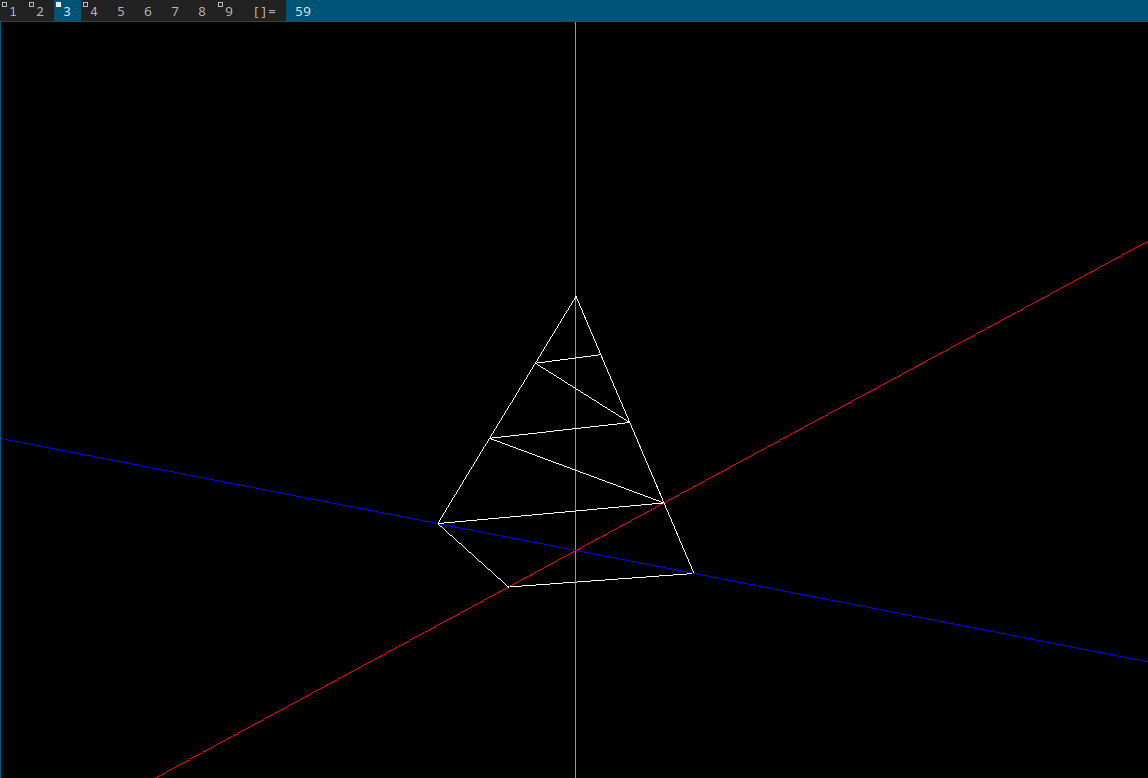
\includegraphics[width=0.5\textwidth]{images/1.png}
\caption{Teste 1}
\end{figure}

\begin{figure}[ht]
\centering
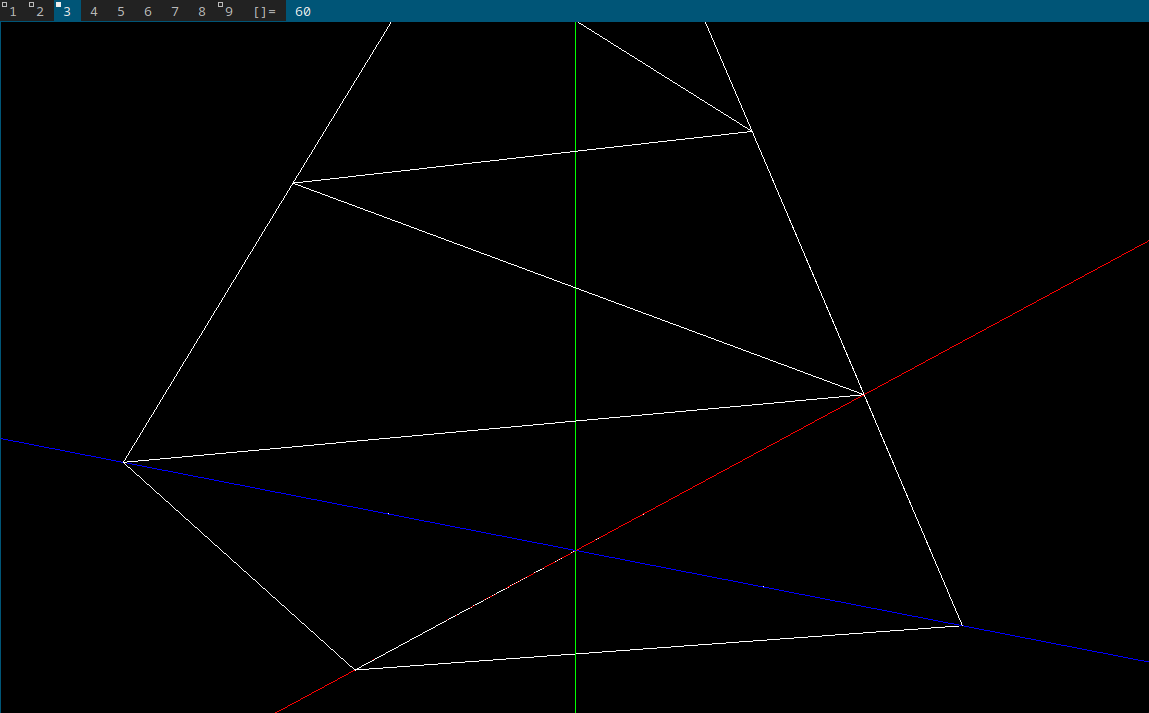
\includegraphics[width=0.5\textwidth]{images/2.png}
\caption{Teste 2}
\end{figure}

\begin{figure}[ht]
\centering
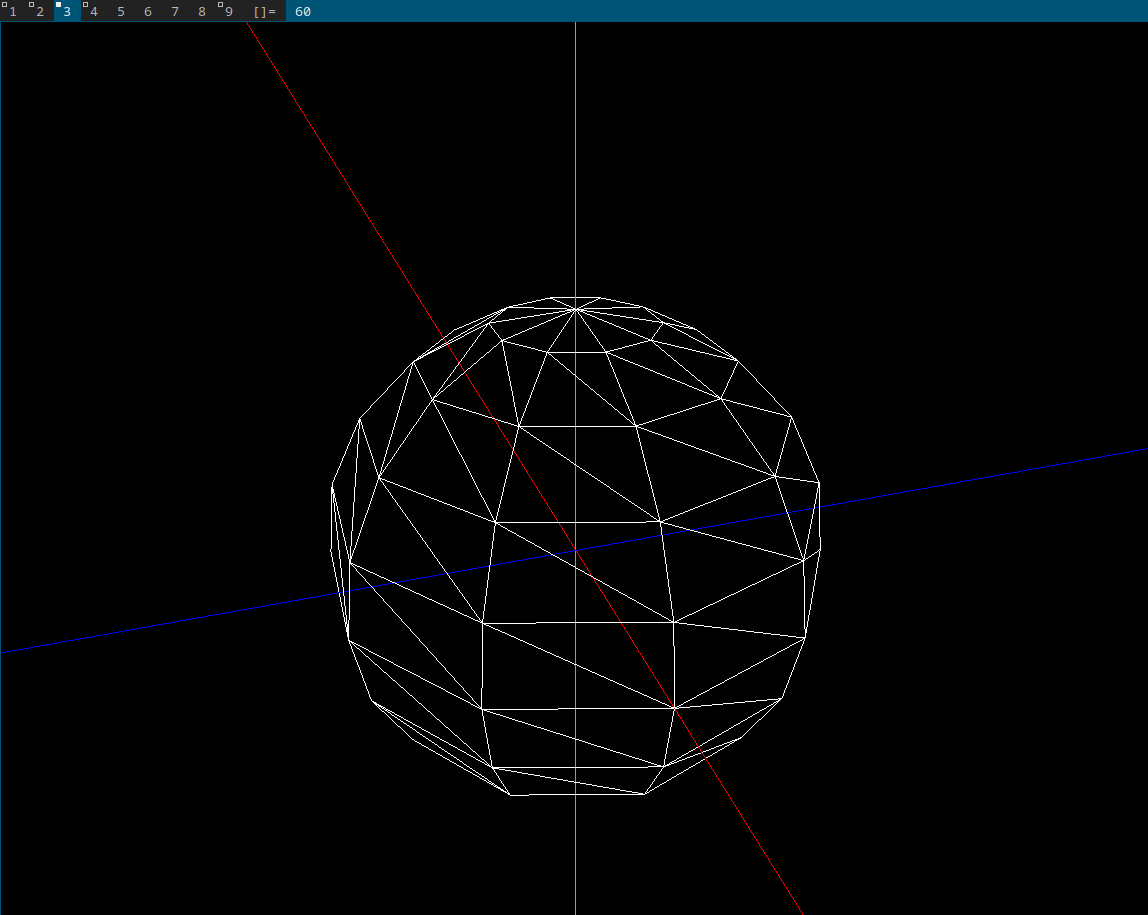
\includegraphics[width=0.5\textwidth]{images/3.png}
\caption{Teste 3}
\end{figure}

\begin{figure}[ht]
\centering
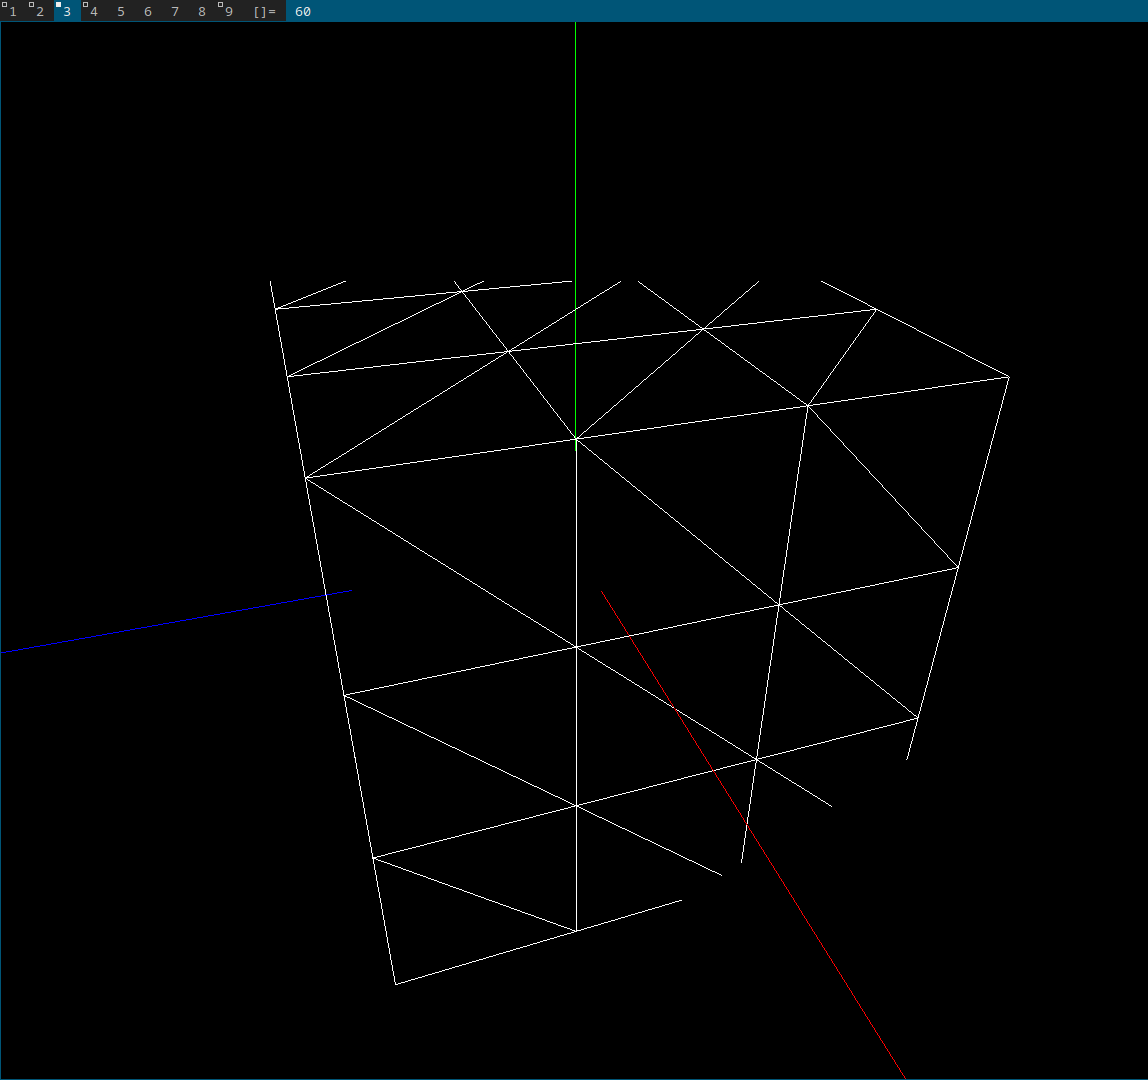
\includegraphics[width=0.5\textwidth]{images/4.png}
\caption{Teste 4}
\end{figure}

\begin{figure}[ht]
\centering
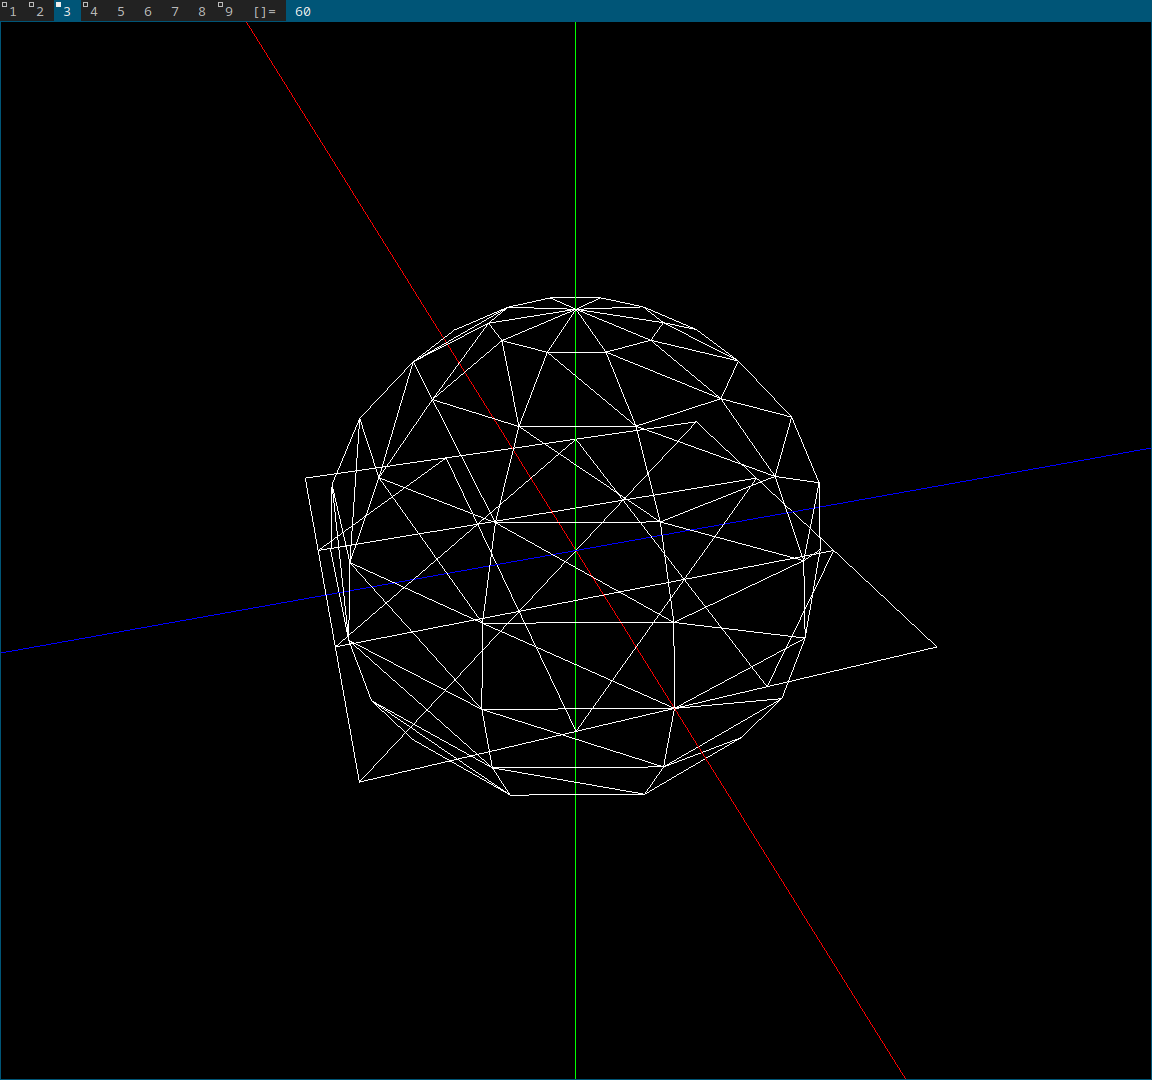
\includegraphics[width=0.5\textwidth]{images/5.png}
\caption{Teste 5}
\end{figure}

\begin{figure}[ht]
\centering
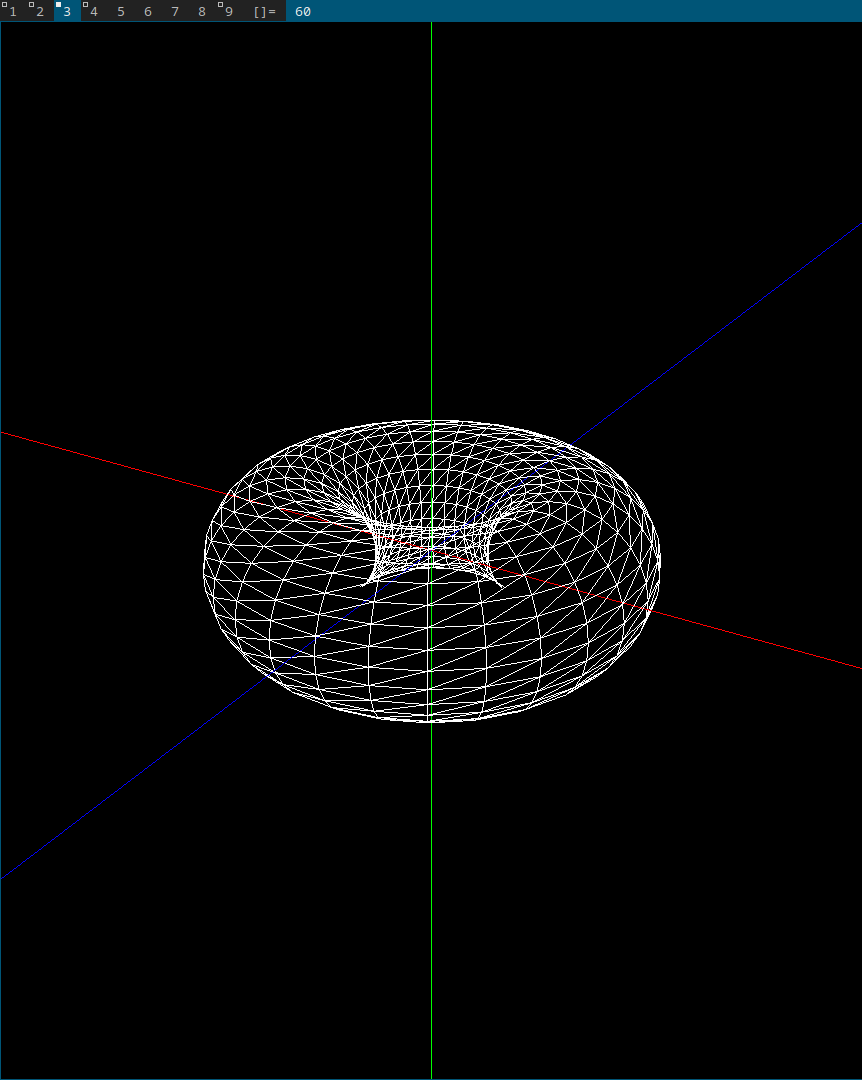
\includegraphics[width=0.5\textwidth]{images/6.png}
\caption{Torus}
\end{figure}


\end{document}
